%chapter 6
\chapter{Freight Transport Operation}
%
Some important terminologies:
\begin{enumerate}
	\item \textbf{\textit{Transport}} is the actual movement of goods from one location to another using a means or a vehicle of transport (e.g. trains, trucks, boats) and a transport infrastructure (e.g. roads, railways, canals).
	\item \textbf{\textit{Distribution}} often denotes all activities relevant to physical movement of goods, including transportation, but also transhipment and warehousing.
	\item \textbf{\textit{Logistics}} is generally used as an overarching term that includes all activities related to the movement and coordination of goods from their source of origin to the final point of delivery, and includes production and distribution. Here, movement does not just correspond to physical movement of goods but also the flow of information.
\end{enumerate}
%
\section{Main Actors of Freight Transport and Distribution}
While freight transport and distribution include many elements, including various organizations and people, the three fundamental actors who actively take part in the domain are described here.
\subsection{Shippers}
The demand for freight transportation is generated by shippers. Each shipper will have their own logistics strategy, which includes whether to operate their own fleet or to use an external party to which it will outsource their logistics and distribution activities, as well as choosing the mode(s) of transport. The process through which the shippers will define their logistics activities generally takes a three-level decision structure:
\begin{enumerate}
	\item The long-term decisions in the first level involve defining strategies in line with their customer network and production activities.
	\item The second-level medium-term decisions include levels of inventories at production, warehousing, and distribution facilities, frequency and amount of shipping and flexibility of service.
	\item At the short-term level, shippers decide on the attributes of the services required for its shipments, such as maximum rates, transport time, reliability and safety.
\end{enumerate}
%
In making these decisions, they will consider the availability and the characteristics of the services offered on the market by carriers and intermediaries, such as freight brokers and third-party logistics providers.
%%
\subsection{Carriers}
Carriers are people, businesses or organisations that operate and offer transportation services for shippers. They may either provide a customised service, where a vehicle or a fleet will be dedicated exclusively to a particular customer, or operate on the basis of consolidation, where each vehicle contains several pieces of freight for different customers with possibly different origins and destinations. In the latter case, carriers generally operate their services according to a published timetable, which prescribes routes, schedules and rates they offer.
%%
\subsection{Intermediaries}
In some cases, the shipper operates their own fleets of vehicles and does not require an external carrier to ship goods on their behalf. In this case, the management of the relevant transportation and distribution is done inhouse. If a shipper does not own a fleet, then it may choose to work directly with one or several carriers.
\paragraph{}
Shippers may alternatively use a freight forwarder, an intermediary person or organization that acts as a third party and manages the shipments on behalf of the shipper by contracting one or several carriers. They also help to identify a suitable mode or a combination of modes for the shipper. Freight forwarders work closely with shippers and carriers, as well as other entities in the transportation network, such as ports or terminals, particularly if they additionally undertake ancillary services such as customs clearance.
%%
\section{Modes of Transportation}
There exist different means of transporting freight over the network, each of which is referred to as a mode of transport. Transportation modes can be differentiated with respect to the type and specification of the vehicle used, the underlying technology, the relevant infrastructure and the nature of the associated operations. The three main modes of transport are air (e.g., cargo planes), land (including road, rail and off-road) and water (e.g., ships in oceans, barges in rivers). Other modes of transport, such as pipelines (e.g., to transport gas) and cable transport (e.g., elevators and cable-cars), also exist.
\paragraph{}
The term mode can also be used to denote different types of vehicles
within a given domain of transport. For example, trucks, vans and bicycles can be seen as three separate modes operating within road transportation due to their distinct features, such as different capacities, capabilities and restrictions. In this example, trucks have the largest capacity but often have restrictions in traveling in urban areas, whereas bicycles are much smaller in capacity but do not suffer from the same type of restrictions as trucks or vans. Brief descriptions of the three main modes of transportation are explained here.
%
\subsection{Road}
Road has been, and continues to be, the most widely used mode of freight transport, both nationally and globally. One of the main reasons behind its popularity is the ability of road transport to offer a very quick service and often be available on demand.
\paragraph{}
A wide variety of vehicles are used for road freight transportation, which
can be differentiated on the basis of size, capacity, weight and the type of energy used. Vehicle classification on road transportation is generally based on the Gross Vehicle Weight Rating (GVWR), which refers to the maximum allowable total weight of a vehicle including its empty mass, fuel and any load carried. The empty mass of the vehicle, but with fuel and fluids such as engine oil, is named as the curb weight. Vehicle classifications vary from one country to another. In the United States, eight classes exist, with vehicles in the lightest class having a GVWR up to around 3 tonnes, and those in the heaviest class with a GVWR higher than 15 tonnes. In the United Kingdom, more classes exist, with those of at most 3.5 tonnes gross weight described as light goods vehicles (LGVs) and those between 3.5 and 44 tonnes gross weight named as lorries or heavy goods vehicles (HGVs).
\paragraph{}
Most vehicles used in road freight transportation run on gasoline or diesel engines. Vehicles using alternative sources of fuel or energy have also been developed, such as those running on batteries, biofuels (such as bioalcohol or ethanol), biodiesel, compressed natural gas, hydrogen, and liquefied petroleum gas (LPG), for use in freight distribution. Within urban areas, human-powered vehicles, such as bicycles and tricycles, can also be used for goods deliveries. To overcome the sole dependency on human power, some of the freight bicycles have power assist motors to aid the cyclist.
\paragraph{}
The road network is composed of motorways (or highways), urban roads,
rural roads, lanes or graded roads and includes bridges and tunnels. Traffic on the road network is controlled by means of traffic signals, signs or markings on the pavement. Various legal requirements are imposed on freight vehicles traveling on the road network, which include limitations on vehicle weight, dimensions, mandatory equipment, licenses and insurances. As for truck drivers, there also exist regulations on driving and working hours, which restrict the duration of driving time and require break and rest periods in long-haul journeys. These regulations aim at reducing driver fatigue, which is known to have adverse affects on road and driver safety. The regulations usually differentiate between on-duty time, which is the time spent working, including driving, waiting, loading and unloading and doing paperwork, and off-duty time, where the driver has no obligation to work. In the United States, for example, these regulations are known as Hours of Service, which limit the maximum consecutive driving time between two rest periods to 11 hours, at which point the driver must be off-duty for at least 10 consecutive hours. Furthermore, a truck driver cannot drive if 8 hours or more have elapsed since the end of the last off-duty period of at least 30 minutes. Similar regulations prevail in other countries, albeit with differences.
%
\subsection{Rail}
Rail freight transportation is known for its ability to offer cost-effective long-haul transportation services, primarily, but not exclusively, for bulk cargo. There are two major components of a rail system, namely the rail network infrastructure and freight trains.
\paragraph{}
The rail network is a large and complex structure composed of nodes and
tracks (or track segments) as links between the nodes. The former include yards or terminals where classification or marshalling operations are performed, stations where cargo is picked up from or delivered to and junctions that are signal-controlled points in the rail network to allow trains to switch from one route to another.
\paragraph{}
Freight trains are composed of one or more locomotives, and several rail
wagons (or cars). Locomotives move the train along the tracks by either pulling it from the front or push from the rear and range from the earlier types powered by steam to contemporary ones using electricity, magnetic force or diesel engine. Rail wagons carry the freight and come in a variety of forms, including specialized wagons for carrying particular types of cargo (e.g., autoracks for carrying automobiles or refrigerator cars for temperature-sensitive goods). A train is characterized by its route, origin, destination, intermediate stops, the physical path it travels on and the schedule information that includes departure and arrival times at each station where it stops. Each wagon also has an itinerary that specifies an origin and a destination station and need not correspond to the origin and destination of the train on which it is carried. Wagons may travel on several trains during their journey, usually in groups called blocks. Each block is assigned an origin and a destination, although individual cars in a single block may have different origins and destinations. A block is treated as a single unit for handling purposes. Once formed at its origin yard, a block will not be classified again until it arrives at its destination yard.
\paragraph{}
Classification or marshalling refers to a set of operations carried out at
yards or terminals, where incoming trains are disassembled by decoupling the rail cars and new trains are formed using individual cars or blocks. Bekta¸s et al. (2009) provide a detailed description of the operations at a classification yard, according to which a train arriving at a yard first enters a receiving area, where the engines are taken away for inspection and maintenance, blocks are separated and cars are inspected. The classification operation begins from this point on and can be performed in two ways, depending on the type of the rail yard. In flat yards, a switching engine is used to push a group of cars out of the receiving tracks onto one of the classification tracks. In hump yards, classification is performed by using an artificially built hill, called the hump, where an engine pushes a group of cars out of the receiving area and up the ramp until it reaches the top of the hill. Due to the pull of the gravitational force, the cars roll down the incline on the other side of the hump, usually one car at a time, and are directed onto one of the classification tracks. Following this operation, each classification track becomes occupied by a group of cars that form the block. Each block then waits until the departure time of its outbound train. When the train is due to leave, they are pulled out of the classification tracks onto the departure tracks and are attached to the train. Following one last inspection of the whole train, the train and blocks leave the yard. The figure below shows the general structure of a classification hump yard.
%
\begin{center}
	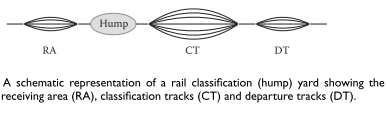
\includegraphics[scale=0.7]{gfx/fig33.png}
\end{center}
\paragraph{}
Classification is not the only operation that is performed at a rail yard.
Other types of operations include inspection, crew change, refueling the trains and dropping and picking up blocks of cars. Among these, however, classification is known to be the major time-consuming operation.
%
\subsection{Air}
Air transportation is mainly used for goods that are time sensitive or have high value-to-weight ratios, including perishables due to the need for speed, fashion goods, emergency supplies and spare parts. Speed is a major advantage of air transportation but comes with the significant drawback of having a very high cost. This is one of the reasons as to why air transport has always had a marginal share in the amount of freight shipped worldwide, in comparison to other modes of transport.
\paragraph{}
Air freight transportation uses a system of air hubs, where outgoing cargo
to be shipped is received and consolidated for shipping to a different hub in the network or incoming cargo from another hub is separated and shipped to its final destination. The network tends to have a hub-and-spoke structure to make the best use of economies of scale and help to achieve the lowest possible cost of transport. Specialized pallets or containers named unit load devices are used to stow cargo in aircraft, in a safe and efficient way. Air cargo can be carried in passenger planes along with passenger baggage. Alternatively, it can be transported in cargo aircraft designed specifically for freight, or by helicopters for access to areas that are difficult to reach.
%
\subsection{Sea}
Sea or maritime transport is the dominant mode with which a large majority of international trade is moved. It is suitable for transporting bulk goods, large packages or containers and similar types of cargo that are not time sensitive.
\paragraph{}
Vessels are the main vehicles of maritime transport, ranging from small
boats to larger ships. Some of the common ship types include break-bulk vessels that are used to transport any type of loose cargo excluding liquid or loose bulk commodities (e.g. boxes, barrels, casks and bagged cargo), Roll-on/Roll-off (RoRo) vessels that carry wheeled cargo (e.g. cars, trucks, trailers), oil tankers that carry crude oil in liquid form, dry bulk vessels that carry bulk goods (e.g. coal, ore, grain) and reefer ships that carry perishable goods that require refrigeration (e.g. fish, meat, fresh produce).
\paragraph{}
The maritime transportation network consists of ports, which are hubs where ships depart from, stop at, or return to, used for loading, unloading and handling cargo. Ports come in different types based on their location and the nature of the cargo they handle. Seaports are the most common. Some ports only work with containerized cargo and include specialized equipment such as a gantry crane used to transfer containers between a vessel and other vehicles of land-based transport, such as trucks and rail wagons, and a stacker that is used to lift and swap containers, as well as perform loading and unloading operations on trucks and wagons.
\paragraph{}
In maritime transportation, there are larger variations in travel as compared with other modes of transport, caused by, for example, weather conditions or congestion at ports. In addition, travel and loading/unloading times are longer, particularly in the case of intercontinental trade.
\paragraph{}
There are three main modes of operation in maritime transportation:
\begin{enumerate}
	\item \textbf{\textit{Liner shipping}} is where vessels operate on regular routes with fixed schedules. The routes and schedules are published in a timetable, similar to bus services for passenger transportation. The routes are fixed, each of which is called a service route. There may be several vessels operating on a given service route, and this depends on the desired frequency over a given period of time (e.g., weekly).
	\item \textbf{\textit{Industrial shipping}} is where the cargo owner operates their own vessel fleet.
	\item \textbf{\textit{Tramp shipping}} is where a carrier operates a fleet of vessels to transport mandatory cargo between specified ports and within a certain time frame for contracted shippers but can also optionally carry spot cargo for other shippers, in order to increase their revenues. Tramp operators will need to decide on whether to accept or reject any spot cargos, which will depend on capacity and timing considerations in the light of the already scheduled routes for mandatory cargo.
\end{enumerate}
%%
\subsection{Intermodal Transportation}
A transportation network is said to be of unimodal type if it only operates a single mode of transport or of multimodal type if it operates at least two different modes of transport. Uni-modal transport cannot take advantage of the use of several modes of transportation, and it is either impractical or impossible to assume a single mode of transport for performing door-to-door delivery. If freight originates from an inland warehouse, for example, and is destined to another inland warehouse on another continent, then part of the journey will have to involve air or water transport.
\paragraph{}
However, even if there are no physical or geographical limitations, carrying small amounts of cargo on a relatively large vehicle from origin to destination is inefficient. One way to improve efficiency is consolidation. The aim of intermodal transportation is exactly this, that is, to consolidate loads for efficient long-haul transportation (e.g., by rail or large ocean vessels), while taking advantage of the efficiency of local pick-up and delivery operations by truck. For any shipment to be intermodal, freight must be transported from origin to destination by a sequence of at least two modes of transport, where transfers from one mode to another take place at intermodal terminals (such as sea ports or rail yards). An illustrative example is provided here.
\\\\
\textit{Example:}\\
\textit{A multimodal transportation network is illustrated in the figure below, on which three modes of transportation, namely road (trucks), rail and water (shipping), operate. Cargo originates from the two facilities seen on the far left of the figure and is destined to the warehouses appearing on the far right of the figure. The figure also shows how the cargo is shipped using an intermodal chain of modes. In particular, loaded trucks leave the origin facilities to a rail yard, where they are consolidated into a train and sent to another rail yard. Trucks are again used to transport the containers from this rail yard to a sea container terminal. This last operation may not be necessary if the sea container terminal has an interface to the rail network, in which case freight is transferred directly from the former onto the latter. Containers are then transported to a port on another continent by ocean shipping, from where they leave by either trucking or rail (or both) to their destinations.}
\begin{center}
	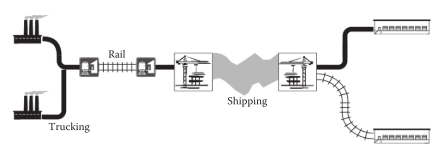
\includegraphics{gfx/fig34.png}
\end{center}
One of the advantages of intermodal freight transport is the possibility of modal shift, which is defined as partially or fully transferring freight from one mode to the other in the network when it is being shipped to its final destination.
%
\subsubsection{Intermodal Terminals}
In intermodal transportation, transfers from one mode to another, and all associated operations related to, for example, loading and unloading, temporary storage or intermediate buffer, and even pre-delivery inspection or enhancement work on the goods are carried out at intermodal terminals. Here are some examples of intermodal terminals:
\begin{itemize}
	\item \textbf{\textit{Rail yards}} where transfers between the two modes of road (e.g. trucks and lorries) and rail take place.
	\item \textbf{\textit{Sea ports}} that act as the interface between sea transport (vessels, ferries) and land transport (road or rail). A barge terminal is a smaller port used in inland river transportation and is linked to larger sea terminals.
	\item \textbf{\textit{Inland distribution}} centers that are used only for road transportation, and act as transfer points between different modes of road transport, for example lorries and vans. Warehouses and cross-docking centres are examples to inland distribution centers.
\end{itemize}
%
\subsubsection{Containerized Transport}
Cargo flow in an intermodal transportation network can be carried by a variety of means, for example crates, pallets or boxes for fresh produce, specialized vessels or tanks for liquid bulk cargo. Irregularity of general cargo, in shape or size, has led to the development of standardized units of shipment, which came to be known as containers. A container is a steel or Aluminium box, with a standard size of 20 ft in length, known as the Twenty Foot Equivalent Unit (TEU), is widely used around the globe, but 40 and 45 ft containers are more commonly used in North America. Containers offer a number of advantages over non-containerized cargo, which are summarized as follows:
\begin{enumerate}
	\item Containers can be locked, which means that their contents cannot easily be modified except at origin or destination, which implies increased safety and reduced loss and damage.
	\item Due to its standard structure, transfer operations at terminals can also be tailored to process containerized cargo fast and with minimal amount of effort. Container ports are excellent examples where such operations can be seen, using container-specific equipment such as container gantry cranes, implying reduced cargo handling.
	\item Containers can be stacked, which implies a more efficient use of storage space within the port.
	\item Cargo of various sizes, shapes, dimensions or weight can be carried in a container, making it a flexible enough means of transport to accommodate for a variety of cargo types.
\end{enumerate}
Due to these advantages, intermodal transportation, as it is implemented and used today, heavily relies on containerization, to the point that intermodal transportation is often equated to moving containers over long distances, on multimodal networks. Intermodal transportation is not restricted, however, to containers and intercontinental exchanges.
%
\section{Choice of Carrier and Transportation Mode}
There are a number of factors that shippers use to decide which particular mode or modes of transportation to use for shipping their freight. Earlier studies on this topic have identified six main factors that influence a shipper’s decision:
\begin{itemize}
	\item Freight rates (including cost and charges)
	\item Reliability (delivery time)
	\item Transit times (time-in-transit, speed, delivery time)
	\item Over, short and damaged shipments (loss, damage, claims processing, tracing)
	\item Shipper market considerations (customer service, user satisfaction, market competitiveness, market influences)
	\item Carrier considerations (availability, capability, reputation, special equipment)
\end{itemize}
Later research identified frequency and flexibility as additional factors in particular industries, and that factors such as international dimension, economies of scale, security, environmental concerns and energy use, integration with the supply chain and information technologies, and particularly the use of the Internet are all relevant to the transportation mode choice but remain as under-researched areas.
\paragraph{}
Other studies have recognized that the perception of a mode of transport
is likely to have a significant effect on the choice of mode. Of the more prominent ones, earlier research has identified communication, quality of service, consistency (in delivery), transit times and rates as being the main factors, with the first two being more significant than the others.
%
\section{Shipment Options}
There are at least two ways in which shipments can be made, which are described in more detail here.
%
\subsection{Direct or Customized Shipments }
Direct or customized shipments arise when goods are shipped from the source of supply to the demand point without the use of any intermediate facilities or demand points. Full-load trucking is an example of customized transportation, where, upon the call of a customer wishing to have goods shipped from one (source) point to another (destination) point, a dispatcher assigns a truck to this task. The truck travels to the customer location, is loaded and then moves to the destination, where it is unloaded. Following this, the driver is assigned a new task by the dispatcher, kept waiting until a new demand appears in the near future, or repositioned to a location where a load exists or is expected to be available about the arrival time. The advantages of full-load trucking come from its flexibility in adapting to a highly dynamic environment and uncertain future demands, offering reliability in service and low tariffs compared to other modes of transportation. The fill efficiency of full-load trucking is achieved through the implementation of resource management and allocation strategies that seek to make the best use of the available resources, while maximizing the volume of demand satisfied and the associated profits. Customized services are also offered, for example, by charted sea or river vessels and planes.
%
\subsection{Consolidated Shipments}
In many cases, trade-offs between volume and frequency of shipping, along with the cost of transportation, render customized services impractical. In such cases, consolidation is used for serving a number of demand points using a particular service. Freight consolidation transportation is performed by Less-Than-Truckload (LTL) motor carriers, railways, ocean shipping lines, regular and express postal services, etc. One example of LTL transportation is when the loads of a given set of customers are consolidated at a given source (e.g. a depot), and the deliveries are multiple destination points. In this case, a truck or a lorry is loaded with all the goods at the depot and is dispatched to visit the customers in a particular order to perform the deliveries. A consolidation-based transportation system can also be structured as a hub-and-spoke network, where shipments for a number of origin-destination points may be transferred via intermediate consolidation facilities, or hubs, such as airports, seaport container terminals, rail yards, truck break-bulk terminals and intermodal platforms.
%
\section{Distribution Structures}
The structure of the way in which goods are distributed is generally in the form of single-echelon (or single-tier) or multi-echelon (or multi-tier) distribution network. The type of structure used depends on a number of factors, such as the type of area (e.g. urban, suburban, rural) or the size of the area (e.g. countries, continents), the type of product(s) being shipped, the types of vehicles used and the demand requirements in terms of volume and time.
\subsection{Single-echelon }
A single-echelon distribution structure does not involve the use of any intermediate facilities between the source(s) of supply and the source(s) of demand and operates on the basis that deliveries are made from the former to the latter. This might be in the form of direct shipments from the supply point to the customer, or, as in the case of consolidation, from one supply point to many customers.
\begin{center}
	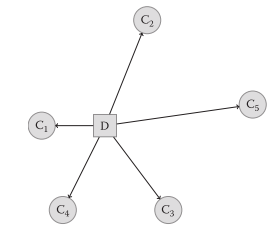
\includegraphics{gfx/fig35.png}
\end{center}
The figure above shows a single echelon distribution structure where a central
depot, shown by $ D $, serves five customers labeled $ C_1–C_5 $, all using direct shipments. In this example, it is assumed that each link carries at least one full-truckload shipment. The figure below shows the same network in which it is assumed that the deliveries can be consolidated. In particular, one LTL vehicle serves customers $ C_1 $ and $ C_4 $ in the given order, and the other serves customers $ C_3 $,$ C_5 $ and $ C_2 $ in the given order.
\begin{center}
	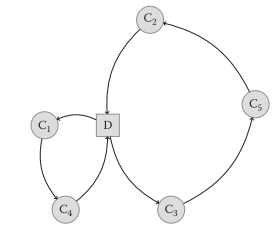
\includegraphics{gfx/fig36.png}
\end{center}
%
\subsection{Multi-echelon}
If the distribution network includes several layers of intermediate facilities, such as warehouses, consolidation facilities, distribution centres and cross-docks, to which the goods are sent as part of the distribution from their origin(s) to their destination(s), then the network is said to have a multi-echelon structure. Supply chain networks often have such a structure, for which the planning problems entail the management and operation of the facilities in the network as well as the assignment of (aggregated) flow between the facilities. In the context of freight distribution, however, the planning problems are more specific to the management of transport modes and the vehicle fleets used in between the different layers.
\begin{center}
	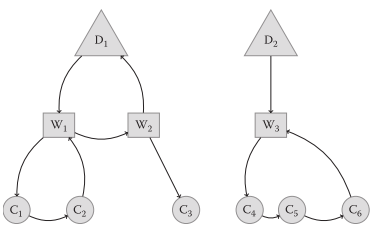
\includegraphics{gfx/fig37.png}
\end{center}
A two-echelon network distribution structure is shown in the figure above, where the first echelon includes all movements between the first layer of depots shown by $ D_1 $ and $ D_2 $ and the second layer of intermediate points (e.g. warehouses) shown by $ W_1 $, $ W_2 $ and $ W_3 $. In this example, consolidated shipments depart from D1 to serve the two warehouses $ W_1 $ and $ W_2 $. In contrast, a direct shipment using a full-truckload is made between $ D_2 $ and $ W_3 $. The second echelon consists of all the distribution activities between the second layer and the third layer, where the latter includes six demand points shown by $ C_1–C_6 $. It is clear from the figure that this network uses a mix of consolidated and direct shipments at this echelon.
\paragraph{}
Structures such as those shown in the figure above have been suggested for use
within urban areas, where the first layer of depots consists of those that are located outside the boundaries of the urban zone and the second layer consists of intermediate points located on the boundaries. The expectation is that bulk deliveries are made from the first to the second layer using heavy goods vehicles, which would stop here. The distribution activities within the urban zone would then be carried out using smaller vehicles that would operate between the second layer of intermediate points and the third layer of demand points. Such a strategy prevents large and heavy vehicles from entering urban zones.
%
\section{Transportation Model}
The transportation model deals with a special class of linear programming problem in which the objective is to transport a homogeneous commodity from various origins or factories to different destinations or markets at a total minimum cost.
%
\subsection{Definition of the Transportation Model}
The problem is represented by the network in the figure below. There are $ m $ sources and $ n $ destinations, each represented by a node. The arcs represent the routes linking the sources and the destinations. Arc $ (m, n) $ joining source $ m $ to destination $ n $ carries two pieces of information: the transportation cost per unit, $ c_{mn} $, and the amount shipped, $ x_{mn} $. The amount of supply at source $ m $ is $ a_m $, and the amount of demand at destination $ n $ is $ b_n $. The objective of the model is to minimize the total transportation cost while satisfying all the supply and demand restrictions.
\begin{center}
	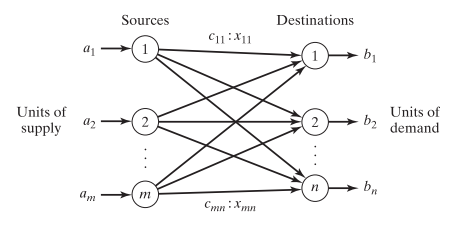
\includegraphics{gfx/fig53.png}
\end{center}
\textit{Example \#1:}\\\\
MG Auto has three plants in Los Angeles, Detroit, and New Orleans and two major distribution centers in Denver and Miami. The quarterly capacities of the three plants are 1000, 1500, and 1200 cars, and the demands at the two distribution centers for the same period are 2300 and 1400 cars. The transportation costs per car on the different routes, rounded to the closest dollar is given in the table below. Determine the amount of cars to distributed to each distribution center such that the cost transportation cost is minimum, satisfying all demand and supply constraints.
\begin{center}
	\begin{tabular}{|c |}
		Transportation cost per car\\
		\hline
		\begin{tabular}{c | c | c}
			From/To & Denver(1) & Miami(2)\\
			\hline
			LA (1) & \$80 & \$215\\
			\hline
			Detroit (2) & \$100 & \$108\\
			\hline
			New Orleans (1) & \$102 & \$68\\
		\end{tabular}
	\end{tabular}
\end{center}
\textit{Solution:}\\\\
The linear Programming model of the problem is:\\\\
Minimize, $ z = 80x_{11} + 215x_{12} + 100x_{21} + 108x_{22} + 102x_{31} + 68x_{32} $\\\\
Subject to:\\
\hspace*{10mm}$x_{11}$ + $x_{12}$ + 0 + 0 + 0 + 0 = 1000 (LA)\\
\hspace*{10mm}0 + 0 + $x_{21}$ + $x_{22}$ + 0 + 0 = 1500 (Detroit)\\
\hspace*{10mm}0 + 0 + 0 + 0 + $x_{31}$ +$x_{32}$ = 1200 (New Orleans)\\
\hspace*{10mm}$x_{11}$ + 0 + $x_{21}$ + 0 + $x_{31}$ + 0 = 2300 (Denver)\\
\hspace*{10mm}0 + $x_{12}$ + 0 + $x_{22}$ + 0 + $x_{32}$ = 1400 (Miami)\\
\hspace*{10mm}$x_{ij} \geq 0$, $i$ = 1, 2, 3 and $j$ = 1, 2\\\\
All the constraints are equations because the total supply ( = 1000+ 1500 + 1200 = 3700) equals the total demand ( = 2300 + 1400 = 3700).
\begin{center}
	\begin{tabular}{c | c | c | c}
		From / To & Denver & Miami & \textbf{Supply}\\
		\hline
		LA & \innerbox{80}{$ x_{11} $} & \innerbox{215}{$ x_{12} $} & 1000\\
		\hline
		Detroit & \innerbox{100}{$ x_{21} $} & \innerbox{108}{$ x_{22} $} & 1500\\
		\hline
		New Orleans & \innerbox{102}{$ x_{31} $} & \innerbox{68}{$ x_{32} $} & 1200\\
		\hline
		\textbf{Demand} & 2300 & 1400 & 	
	\end{tabular}
\end{center}
The special structure of the transportation problem allows a compact representation of the problem using the transportation tableau format in shown above.\\\\
The optimal solution of the given transportation problem ships 1000 cars from LA to Denver ( $ x_{11} = 1000 $), 1300 from Detroit to Denver ( $ x_{21} = 1300 $), 200 from Detroit to Miami ( $ x_{22} = 200 $), and 1200 from New Orleans to Miami ( $ x_{31} = 1200 $). The associated minimum transportation cost is computed as $ 100 \times \$80 + 1300 \times \$100 + 200 \times \$108 + 1200 \times \$68 = \$313,200$.\\\\
A transportation problem is said to be balanced if the total supply equals to the total demand. However, if the problem is not balanced then it can be balanced by introducing a dummy row or column having cost value of zero, i.e:
\begin{itemize}
	 \item \textbf{\textit{If Total Supply $<$ Total Demand:}} A dummy row, whose each cell have zero cost value, is added to the table with a corresponding supply value = Total Demand - Total Supply.
	 \item \textbf{\textit{If Total Supply $ > $ Total Demand:}} A dummy column, whose each cell have zero cost value, is added to the table with a corresponding demand value = Total Supply - Total Demand.
\end{itemize}
%
\subsection{The Transportation Algorithm}
The special transportation algorithm that will be presented in this section was developed early on when hand computations were the norm and shortcuts were warranted. Today, powerful computer codes can solve transportation models of any size as a regular LP. But there is more to the transportation model than the hand computations. First, its historical significance in the evolution of OR techniques is important and must be preserved. Second, the special transportation tableau format can facilitate modeling a number of situations that do not deal directly with transporting goods. Third, the algorithmic hand computations boast such (almost intuitive) simplicity that a beginner can get a “feel” of what optimization is about. Lastly, the transportation algorithm does provide insight into the use of the theoretical primal–dual relationships to achieve a practical end result—that of developing simple rules for hand computations. The exercise is theoretically intriguing.\\\\
The basic steps of the Transportation Algorithm are as follows:
\begin{itemize}
	\item \textbf{Step 1}: Balance the given transportation problem.
	\item \textbf{Step 2}: Compute the starting basic feasible solution. A basic feasible solution can be computed using either of these methods:
	\begin{enumerate}
		\item North - west corner method.
		\item Least - cost cell method. (Or Inspection method Or Matrix minimum - row minimum - column minimum method).
		\item Vogel's Approximation Method, generally known as VAM.
	\end{enumerate}
	\item \textbf{Step 3}: After getting the basic feasible solution conduct a optimality test to check whether the solution is optimal or not. There are two methods of computing optimality test, they are:
	\begin{enumerate}
		\item Stepping Stone Method.
		\item Modified Distribution Method, generally known as MODI method.
	\end{enumerate}
\end{itemize}
For this subject, we will be only computing up to the basic feasible solution of the transportation problem since solving for optimality test is a cumbersome task on its own and doing so causes to deviate away from the course domain of the subject. These topics are only introduced for the sake of familiarizing students with the scope of transportation engineering. For an in-depth study about these topics, students are highly encouraged to peruse books related to Operation Research.
%
\subsection{Determining the Basic Feasible Solution}
%
\subsubsection{a. North-West Corner Method}
The following are the steps used for determining the basic feasible solution of a transportation problem using the North-West Corner Method:
\begin{itemize}
	\item Balance the problem, that is, check whether the total demand is equal to the total demand or not. If not, open a dummy column or dummy row as the case may be and balance the problem.
	\item Start from the left hand side top corner or cell and make allocations depending on the availability and requirement constraint. If the availability constraint is less than the requirement constraint, then for that cell make allocation in units which is equal to the availability constraint. In general, verify which is the smallest among the availability and requirement and allocate the smallest one to the cell under question. Then proceed allocating either side ways or downward to satisfy the rim requirement. Continue this until all the allocations are over.
	\item Once all the allocations are over, i.e., both rim requirement (column and row i.e., availability and requirement constraints) are satisfied, write allocations and calculate the cost of transportation.
\end{itemize}
\textbf{\textit{Numerical Example:(Sunray Transport Problem)}}\\
SunRay Transport Company ships truckloads of grain from three silos to four mills. The supply (in truckloads) and the demand (also in truckloads) together with the unit transportation costs per truckload on the different routes are summarized in the table below. The unit transportation costs are in hundreds of dollars. The model seeks the minimum cost shipping schedule between the silos and the mills.
\begin{center}
	\begin{tabular}{c}
		Transportation Cost\\
		 \hline
		\begin{tabular}{c | c | c | c | c | c}
			Silo / Mill \cellcolor{cyan} & 1 \cellcolor{cyan} & 2 \cellcolor{cyan} & 3 \cellcolor{cyan} & 4 \cellcolor{cyan} & Supply \cellcolor{cyan}\\
			\hline
			1 \cellcolor{cyan} & \$10 & \$2 & \$20 & \$11 & 15\\
			\hline
			2 \cellcolor{cyan} & \$12 & \$7 & \$9 & \$20 & 25\\
			\hline
			3 \cellcolor{cyan} & \$4 & \$14 & \$16 & \$18 & 10\\
			\hline
			Demand \cellcolor{cyan} & 5 & 15 & 15 & 15 & 
		\end{tabular}
	\end{tabular}
\end{center}
\textit{Solution:}\\
Total Supply = 15 + 25 + 10 = 50\\
Total Demand = 5 + 15 + 15 + 15 = 50\\\\
$\because$ Total Supply = Total Demand, the transportation model is balanced.\\\\
At first, we choose the cell that is in the extreme north-west position, that is, cell corresponding to transport operation from silo 1 to mill 1. For that cell, we have supply of 15 and demand of 5. $ \because 5 < 15$, we allocate the value of 5 this cell. Allocating 5 truckloads from silo 1 to mill 1 leaves silo 1 with a remainder of 10 truckloads of supply. Also demand for mill 1 has been satisfied so we gray out the column corresponding to mill 1 indicating it requires no further action. This is shown in the transportation tableau below:
\begin{center}
	\begin{tabular}{c | c | c | c | c | c}
		Silo / Mill & 1 & 2 & 3 & 4 & \textbf{Supply}\\ 
		\hline
		1 & \innerbox{\$10}{5} \cellcolor[gray]{0.8} & \$2 & \$20 & \$11 & $ \cancel{15} $ 10\\
		\hline
		2 & \$12 \cellcolor[gray]{0.8} & \$7 & \$9 & \$20 & 25\\
		\hline
		3 & \$4 \cellcolor[gray]{0.8} & \$14 & \$16 & \$18 & 10\\
		\hline
		Demand & $ \cancel{5} $ & 15 & 15 & 15 & \\
		 & 0 & & & & 
	\end{tabular}
\end{center}
Similarly, cell corresponding to transport operation from silo 1 to mill 2 is in the north-west position considering the remaining table (Table excludes the grayed out region). For this cell, supply is 10 and demand is 15. $\because 10 < 15$, we allocate value of 10 for this cell. Allocating 10 truckloads from silo 1 leaves the supply capacity of silo 1 to 0 and demand of mill 2 is reduced to 5 truckloads. Since silo 1 can no longer supply any truckloads, we gray out the corresponding row.
\begin{center}
	\begin{tabular}{c | c | c | c | c | c}
		Silo / Mill & 1 & 2 & 3 & 4 & \textbf{Supply}\\ 
		\hline
		1 & \innerbox{\$10}{5} \cellcolor[gray]{0.8} & \innerbox{\$2}{10} \cellcolor[gray]{0.8} & \$20 \cellcolor[gray]{0.8} & \$11 \cellcolor[gray]{0.8} & $ \cancel{15} $ $ \cancel{10} $ 0\\
		\hline
		2 & \$12 \cellcolor[gray]{0.8} & \$7 & \$9 & \$20 & 25\\
		\hline
		3 & \$4 \cellcolor[gray]{0.8} & \$14 & \$16 & \$18 & 10\\
		\hline
		Demand & $ \cancel{5} $ & $ \cancel{15} $ & 15 & 15 & \\
		& 0 & 5 & & & 
	\end{tabular}
\end{center}
Similarly, cell corresponding to transport operation from silo 2 to mill 2 is in the north-west position considering the remaining table. For this cell, supply is 25 and demand is 5. $\because 5 < 25$, we allocate value of 5 for this cell. Allocating 5 truckloads from silo 2 reduces the supply capacity of silo 2 to 20 and demand of mill 2 is reduced to 0 truckloads. Since mill 2 can no longer receive truckloads, we gray out the corresponding column.
\begin{center}
	\begin{tabular}{c | c | c | c | c | c}
		Silo / Mill & 1 & 2 & 3 & 4 & \textbf{Supply}\\ 
		\hline
		1 & \innerbox{\$10}{5} \cellcolor[gray]{0.8} & \innerbox{\$2}{10} \cellcolor[gray]{0.8} & \$20 \cellcolor[gray]{0.8} & \$11 \cellcolor[gray]{0.8} & $ \cancel{15} $ $ \cancel{10} $ 0\\
		\hline
		2 & \$12 \cellcolor[gray]{0.8} & \innerbox{\$7}{5} \cellcolor[gray]{0.8} & \$9 & \$20 & $ \cancel{25} $ 20\\
		\hline
		3 & \$4 \cellcolor[gray]{0.8} & \$14 \cellcolor[gray]{0.8} & \$16 & \$18 & 10\\
		\hline
		Demand & $ \cancel{5} $ & $ \cancel{15} $ & 15 & 15 & \\
		& 0 & $ \cancel{5}$ & & & \\ 
		&  & 0 & & & \\
	\end{tabular}
\end{center}
Similarly, cell corresponding to transport operation from silo 2 to mill 3 is in the north-west position considering the remaining table. For this cell, supply is 20 and demand is 15. $\because 15 < 20$, we allocate value of 15 for this cell. Allocating 15 truckloads from silo 2 reduces the supply capacity of silo 2 to 5 and demand of mill 3 is reduced to 0 truckloads. Since mill 3 can no longer receive truckloads, we gray out the corresponding column.
\begin{center}
	\begin{tabular}{c | c | c | c | c | c}
		Silo / Mill & 1 & 2 & 3 & 4 & \textbf{Supply}\\ 
		\hline
		1 & \innerbox{\$10}{5} \cellcolor[gray]{0.8} & \innerbox{\$2}{10} \cellcolor[gray]{0.8} & \$20 \cellcolor[gray]{0.8} & \$11 \cellcolor[gray]{0.8} & $ \cancel{15} $ $ \cancel{10} $ 0\\
		\hline
		2 & \$12 \cellcolor[gray]{0.8} & \innerbox{\$7}{5} \cellcolor[gray]{0.8} & \innerbox{\$9}{15} \cellcolor[gray]{0.8} & \$20 & $ \cancel{25} $ $ \cancel{20} $ 5\\
		\hline
		3 & \$4 \cellcolor[gray]{0.8} & \$14 \cellcolor[gray]{0.8} & \$16 \cellcolor[gray]{0.8} & \$18 & 10\\
		\hline
		Demand & $ \cancel{5} $ & $ \cancel{15} $ & $ \cancel{15} $ & 15 & \\
		& 0 & $ \cancel{5}$ & 0 & & \\ 
		&  & 0 & & & \\
	\end{tabular}
\end{center}
Similarly, cell corresponding to transport operation from silo 2 to mill 4 is in the north-west position considering the remaining table.  For this cell, supply is 5 and demand is 15. $\because 5 < 15$, we allocate value of 5 for this cell. Allocating 5 truckloads from silo 2 reduces the supply capacity of silo 2 to 0 and demand of mill 3 is reduced to 10 truckloads. Since, silo 2 can no longer supply any truckloads, we gray out the corresponding row.
\begin{center}
	\begin{tabular}{c | c | c | c | c | c}
		Silo / Mill & 1 & 2 & 3 & 4 & \textbf{Supply}\\ 
		\hline
		1 & \innerbox{\$10}{5} \cellcolor[gray]{0.8} & \innerbox{\$2}{10} \cellcolor[gray]{0.8} & \$20 \cellcolor[gray]{0.8} & \$11 \cellcolor[gray]{0.8} & $ \cancel{15} $ $ \cancel{10} $ 0\\
		\hline
		2 & \$12 \cellcolor[gray]{0.8} & \innerbox{\$7}{5} \cellcolor[gray]{0.8} & \innerbox{\$9}{15} \cellcolor[gray]{0.8} & \innerbox{\$20}{5} \cellcolor[gray]{0.8} & $ \cancel{25} $ $ \cancel{20} $ $ \cancel{5} $ 0\\
		\hline
		3 & \$4 \cellcolor[gray]{0.8} & \$14 \cellcolor[gray]{0.8} & \$16 \cellcolor[gray]{0.8} & \$18 & 10\\
		\hline
		Demand & $ \cancel{5} $ & $ \cancel{15} $ & $ \cancel{15} $ & $ \cancel{15} $ & \\
		& 0 & $ \cancel{5}$ & 0 & 10 & \\ 
		&  & 0 & & & \\
	\end{tabular}
\end{center}
Finally, there is only one cell left, cell corresponding to transport operation from silo 3 to mill 4, so we assign the remaining 10 truckloads to this cell and the transportation supply and demand constraints are also met.\\\\
From the basic feasible solution obtained using the North-West Corner method, following assignments are obtained: $ x_{11} = 5$, $ x_{12} = 10$, $ x_{22} = 5$, $ x_{23} = 15$, $ x_{24} = 5$, and $ x_{34} = 10$.\\\\
Also, the associated cost of the schedule is,\\
$ z = 5 \times \$10 + 10 \times \$2 + 5 \times \$7 + 15 \times \$9 + 5 \times \$20 + 10 \times \$18 = \$520$
\subsubsection{b. Least-Cost Cell Method}
The least-cost method finds a better starting solution by targeting the cheapest routes. It assigns as much as possible to the cell with the smallest unit cost (ties are broken arbitrarily). Next, the satisfied row or column is crossed out and the amounts of supply and demand are adjusted accordingly. If both a row and a column are satisfied simultaneously, only one is crossed out, the same as in the northwest-corner method. Next, select the uncrossed-out cell with the smallest unit cost and repeat the process until exactly one row or column is left uncrossed out.\\\\
The following are the steps used for determining the basic feasible solution of a transportation problem using the Least-Cost Cell Method:
\begin{itemize}
	\item \textit{Step 1:} Identify the lowest cost cell in the given matrix. When more than one cell has the same cost, then both the cells are competing for allocation. This situation in transportation problem is known as tie. To break the tie, select any one cell of your choice for allocation. Make allocations to this cell either to satisfy availability constraint or requirement constraint. Once one of these is satisfied, then mark crosses (×) in all the cells in the row or column which ever has completely allocated.
	\item \textit{Step 2:} Are all allocations completed? If yes the basic solution has been obtained, else go to the \textit{Step 1.}
\end{itemize}
\textbf{\textit{Numerical Example: Determine the basic feasible solution for the Sunray Transport Problem using the Least-Cost Cell method.}}\\
\textit{Solution:}\\
Total Supply = 15 + 25 + 10 = 50\\
Total Demand = 5 + 15 + 15 + 15 = 50\\\\
$\because$ Total Supply = Total Demand, the transportation model is balanced.\\\\
First, we have to choose the cell having the least cost, in this problem the cell corresponding to transport operation from silo 1 to mill 2 has the least cost (\$2). For this cell, the supply is 15 and demand is also 15. So we assign the value of 15 for this cell, which reduces the supply of silo 1 to 0 and demand of mill 2 to 0. Since silo 1 can no longer supply and mill 2 can no longer receive truckloads, we gray out the corresponding row and column.
\begin{center}
	\begin{tabular}{c | c | c | c | c | c}
		Silo / Mill & 1 & 2 & 3 & 4 & \textbf{Supply}\\ 
		\hline
		1 & \$10 \cellcolor[gray]{0.8} & \innerbox{\$2}{15} \cellcolor[gray]{0.8} & \$20 \cellcolor[gray]{0.8} & \$11 \cellcolor[gray]{0.8} & $ \cancel{15} $ 0\\
		\hline
		2 & \$12 & \$7 \cellcolor[gray]{0.8} & \$9 & \$20 & 25\\
		\hline
		3 & \$4 & \$14 \cellcolor[gray]{0.8} & \$16 & \$18 & 10\\
		\hline
		Demand & 5 & $ \cancel{15} $ & 15 & 15 & \\
		&  & 0 & & & 
	\end{tabular}
\end{center}
Similarly for the remaining active cells, the cell corresponding to transport operation from silo 3 to mill 1 has the least cost (\$4) among other active cells. For this cell, the supply is 10 and demand is 5. Since $ 5 < 10 $ we assign the value of 5 for this cell, which reduces the supply of silo 3 to 5 and demand of mill 1 to 0. Since mill 1 can no longer receive truckloads, we gray out the corresponding column.
\begin{center}
	\begin{tabular}{c | c | c | c | c | c}
		Silo / Mill & 1 & 2 & 3 & 4 & \textbf{Supply}\\ 
		\hline
		1 & \$10 \cellcolor[gray]{0.8} & \innerbox{\$2}{15} \cellcolor[gray]{0.8} & \$20 \cellcolor[gray]{0.8} & \$11 \cellcolor[gray]{0.8} & $ \cancel{15} $ 0\\
		\hline
		2 & \$12 \cellcolor[gray]{0.8} & \$7 \cellcolor[gray]{0.8} & \$9 & \$20 & 25\\
		\hline
		3 & \innerbox{\$4}{5} \cellcolor[gray]{0.8} & \$14 \cellcolor[gray]{0.8} & \$16 & \$18 & $ \cancel{10} $ 5\\
		\hline
		Demand & $ \cancel{5} $ & $ \cancel{15} $ & 15 & 15 & \\
		& 0 & 0 & & & 
	\end{tabular}
\end{center}
Similarly for the remaining active cells, the cell corresponding to transport operation from silo 2 to mill 3 has the least cost (\$9) among other active cells. For this cell, the supply is 25 and demand is 15. Since $ 15 < 25 $ we assign the value of 15 for this cell, which reduces the supply of silo 2 to 10 and demand of mill 3 to 0. Since mill 3 can no longer receive truckloads, we gray out the corresponding column.
\begin{center}
	\begin{tabular}{c | c | c | c | c | c}
		Silo / Mill & 1 & 2 & 3 & 4 & \textbf{Supply}\\ 
		\hline
		1 & \$10 \cellcolor[gray]{0.8} & \innerbox{\$2}{15} \cellcolor[gray]{0.8} & \$20 \cellcolor[gray]{0.8} & \$11 \cellcolor[gray]{0.8} & $ \cancel{15} $ 0\\
		\hline
		2 & \$12 \cellcolor[gray]{0.8} & \$7 \cellcolor[gray]{0.8} & \innerbox{\$9}{15} \cellcolor[gray]{0.8} & \$20 & $ \cancel{25} $ 10\\
		\hline
		3 & \innerbox{\$4}{5} \cellcolor[gray]{0.8} & \$14 \cellcolor[gray]{0.8} & \$16 \cellcolor[gray]{0.8} & \$18 & $ \cancel{10} $ 5\\
		\hline
		Demand & $ \cancel{5} $ & $ \cancel{15} $ & $ \cancel{15} $ & 15 & \\
		& 0 & 0 & 0 & & 
	\end{tabular}
\end{center}
Similarly for the remaining active cells, the cell corresponding to transport operation from silo 3 to mill 4 has the least cost (\$18) among other active cells. For this cell, the supply is 5 and demand is 15. Since $ 5 < 15 $ we assign the value of 5 for this cell, which reduces the supply of silo 3 to 0 and demand of mill 4 to 10. Since silo 3 can no longer supply truckloads, we gray out the corresponding row.
\begin{center}
	\begin{tabular}{c | c | c | c | c | c}
		Silo / Mill & 1 & 2 & 3 & 4 & \textbf{Supply}\\ 
		\hline
		1 & \$10 \cellcolor[gray]{0.8} & \innerbox{\$2}{15} \cellcolor[gray]{0.8} & \$20 \cellcolor[gray]{0.8} & \$11 \cellcolor[gray]{0.8} & $ \cancel{15} $ 0\\
		\hline
		2 & \$12 \cellcolor[gray]{0.8} & \$7 \cellcolor[gray]{0.8} & \innerbox{\$9}{15} \cellcolor[gray]{0.8} & \$20 & $ \cancel{25} $ 10\\
		\hline
		3 & \innerbox{\$4}{5} \cellcolor[gray]{0.8} & \$14 \cellcolor[gray]{0.8} & \$16 \cellcolor[gray]{0.8} & \innerbox{\$18}{5} \cellcolor[gray]{0.8} & $ \cancel{10} $ $ \cancel{5} $ 0\\
		\hline
		Demand & $ \cancel{5} $ & $ \cancel{15} $ & $ \cancel{15} $ & $ \cancel{15} $ & \\
		& 0 & 0 & 0 & 10 & 
	\end{tabular}
\end{center}
Finally the cell corresponding to transport operation from silo 2 to mill 4 is only left which has a both demand and supply value of 10. Hence we assign the value of 10 to this cell.\\\\
From the basic feasible solution obtained using the North-West Corner method, following assignments are obtained: $ x_{13} = 5, x_{12} = 15, x_{23} = 15, x_{24} = 10, and \: x_{34} = 5$.\\\\
Also, the associated cost of the schedule is,\\
$ z = 15 \times \$2 + 5 \times \$4 + 15 \times \$9 + 10 \times \$20 + 5 \times \$18 = \: \$475$.
%
\subsubsection{c. Vogel's Approximation Method (Opportunity Cost Method)}
VAM is an improved version of the least-cost method that generally, but not always, produces better starting solutions. In this method, we use concept of opportunity cost. Opportunity cost is the penalty for not taking correct decision. This is the penalty for not taking correct decision and hence the opportunity cost.
The following are the steps used for determining the basic feasible solution of a transportation problem using the Least-Cost Cell Method:
\begin{itemize}
	\item Step 1: For each row (column), determine a penalty measure by subtracting the smallest unit cost in the row (column) from the next smallest unit cost in the same row (column). This penalty is actually a measure of lost opportunity one forgoes if the smallest unit cost cell is not chosen.
	\item Identify the row or column with the largest penalty, breaking ties arbitrarily. Allocate as much as possible to the variable with the least unit cost in the selected row or column. Adjust the supply and demand, and cross out the satisfied row or column. If a row and a column are satisfied simultaneously, only one of the two is crossed out, and the remaining row (column) is assigned zero supply (demand).
	\item \begin{enumerate}
		\item If exactly one row or column with zero supply or demand remains uncrossed out, stop.
		\item If one row (column) with positive supply (demand) remains uncrossed out, determine the basic variables in the row (column) by the least-cost method. Stop.
		\item If all the uncrossed-out rows and columns have (remaining) zero supply and demand, determine the zero basic variables by the least-cost method. Stop.
		\item Otherwise, go to step 1.
	\end{enumerate}
\end{itemize}
\textbf{\textit{Numerical Example: Determine the basic feasible solution for the Sunray Transport Problem using the Vogel's Approximation method.}}\\
\textit{Solution:}\\
Total Supply = 15 + 25 + 10 = 50\\
Total Demand = 5 + 15 + 15 + 15 = 50\\\\
$\because$ Total Supply = Total Demand, the transportation model is balanced.\\\\
At first, we compute the values of penalties for each row and column of the transportation model. For first row (supply row of silo 1), 10 and 2 are the two minimum values. Thus, the value of penalty for the corresponding row is 8. For first column (demand column of mill 1), 10 and 4 are the two minimum value. Thus, the value of penalty for the corresponding column is 6. Similarly the value of penalty for all rows and columns are computed as shown in the table below. Comparing the values of penalty of all rows and column, it is found that the value of penalty corresponding to the third row, that is 10, is the maximum value. Since 10 is the max value, we determine the cell to be assigned for the corresponding row using least-cost cell method.
\begin{center}
	\begin{tabular}{c | c | c | c | c | c | c}
		S/M & 1 & 2 & 3 & 4 & Supply & $P_1$ \\
		\hline
		1 & \$10 \cellcolor[gray]{0.8} & \$2 & \$20 & \$11 & 15 & 10 - 2 = 8\\
		\hline
		2 & \$12 \cellcolor[gray]{0.8} & \$7 & \$9 & \$20 & 25 & 9 - 7 = 2\\
		\hline
		3 & \innerbox{\$4}{5} \cellcolor[gray]{0.8} & \$14 & \$16 & \$18 & $ \cancel{10} $ 5 & 14 - 4 = 10 $\leftarrow$\\
		\hline
		Demand & $ \cancel{5} $ & 15 & 15 & 15 & & \\
		 & $ 0 $ &  &  &  & & \\
		 \hline
		 $P_1$ & 10 - 4 = 6 & 5 & 7 & 7 & & \\
	\end{tabular}
\end{center}
Similarly, we compute the value of penalty for all active rows and columns. Since 9, which is the penalty value for row 1, is the maximum value among all values of penalty, we determine the cell to be assigned for the corresponding row using least-cost cell method.
\begin{center}
	\begin{tabular}{c | c | c | c | c | c | c | c}
		S/M & 1 & 2 & 3 & 4 & Sup & $P_1$ & $P_2$ \\
		\hline
		1 & \$10 \cellcolor[gray]{0.8} & \innerbox{\$2}{15} \cellcolor[gray]{0.8} & \$20 \cellcolor[gray]{0.8} & \$11 \cellcolor[gray]{0.8} & $ \cancel{15} $ 0 & 8 & 9 $\leftarrow$\\
		\hline
		2 & \$12 \cellcolor[gray]{0.8} & \$7 \cellcolor[gray]{0.8} & \$9 & \$20 & 25 & 2 & 2\\
		\hline
		3 & \innerbox{\$4}{5} \cellcolor[gray]{0.8} & \$14 \cellcolor[gray]{0.8} & \$16 & \$18 & $ \cancel{10} $ 5 & 10 $\leftarrow$ & 2\\
		\hline
		Dem & $ \cancel{5} $ & $ \cancel{15} $ & 15 & 15 & & &\\
		& $ 0 $ & 0 &  &  & & &\\
		\hline
		$P_1$ & 6 & 5 & 7 & 7 & & &\\
		\hline
		$P_2$ & - & 5 & 7 & 7 & & &\\
	\end{tabular}
\end{center}
Similarly,
\begin{center}
	\begin{tabular}{c | >{\small} c | >{\small} c | >{\small} c | >{\small} c | >{\small} c | >{\small} c | >{\small} c | >{\small} c}
		S/M & 1 & 2 & 3 & 4 & Sup & $P_1$ & $P_2$ & $P_3$\\
		\hline
		1 & \$10 \cellcolor[gray]{0.8} & \innerbox{\$2}{15} \cellcolor[gray]{0.8} & \$20 \cellcolor[gray]{0.8} & \$11 \cellcolor[gray]{0.8} & $ \cancel{15} $ 0 & 8 & 9 $\leftarrow$ & -\\
		\hline
		2 & \$12 \cellcolor[gray]{0.8} & \$7 \cellcolor[gray]{0.8} & \innerbox{\$9}{15} \cellcolor[gray]{0.8} & \$20 & $ \cancel{25} $ 10 & 2 & 2 & 11 $\leftarrow$\\
		\hline
		3 & \innerbox{\$4}{5} \cellcolor[gray]{0.8} & \$14 \cellcolor[gray]{0.8} & \$16 \cellcolor[gray]{0.8} & \$18 & $ \cancel{10} $ 5 & 10 $\leftarrow$ & 2 & 2\\
		\hline
		Dem & $ \cancel{5} $ & $ \cancel{15} $ & $ \cancel{15} $ & 15 & & & &\\
		& $ 0 $ & 0 & 0 &  & & & &\\
		\hline
		$P_1$ & 6 & 5 & 7 & 7 & & & &\\
		\hline
		$P_2$ & - & 5 & 7 & 7 & & & &\\
		\hline
		$P_3$ & - & - & 7 & 2 & & & &\\
	\end{tabular}
\end{center}
Similarly,
\begin{center}
	\begin{tabular}{ >{\tiny}c | >{\tiny} c | >{\tiny} c | >{\tiny} c | >{\tiny} c |>{\tiny} c | >{\tiny} c | >{\tiny} c | >{\tiny} c | >{\tiny} c}
		S/M & 1 & 2 & 3 & 4 & Sup & $P_1$ & $P_2$ & $P_3$ & $P_4$\\
		\hline
		1 & \$10 \cellcolor[gray]{0.8} & \innerbox{\$2}{15} \cellcolor[gray]{0.8} & \$20 \cellcolor[gray]{0.8} & \$11 \cellcolor[gray]{0.8} & $ \cancel{15} $ 0 & 8 & 9 $\leftarrow$ & - & -\\
		\hline
		2 & \$12 \cellcolor[gray]{0.8} & \$7 \cellcolor[gray]{0.8} & \innerbox{\$9}{15} \cellcolor[gray]{0.8} & \innerbox{\$20}{10} \cellcolor[gray]{0.8} & $ \cancel{25} $ $ \cancel{10} $ 0 & 2 & 2 & 11 $\leftarrow$ & 20 $\leftarrow$\\
		\hline
		3 & \innerbox{\$4}{5} \cellcolor[gray]{0.8} & \$14 \cellcolor[gray]{0.8} & \$16 \cellcolor[gray]{0.8} & \$18 & $ \cancel{10} $ 5 & 10 $\leftarrow$ & 2 & 2 & 18\\
		\hline
		Dem & $ \cancel{5} $ & $ \cancel{15} $ & $ \cancel{15} $ & $ \cancel{15} $ & & & & &\\
		& $ 0 $ & 0 & 0 & 5 & & & & &\\
		\hline
		$P_1$ & 6 & 5 & 7 & 7 & & & & &\\
		\hline
		$P_2$ & - & 5 & 7 & 7 & & & & &\\
		\hline
		$P_3$ & - & - & 7 & 2 & & & & &\\
		\hline
		$P_4$ & - & - & - & 2 & & & & &\\
	\end{tabular}
\end{center}
The basic feasible solution is shown below:
\begin{center}
	\begin{tabular}{c | c | c | c | c | c}
		Silo / Mill & 1 & 2 & 3 & 4 & Supply \\
		\hline
		1 & 10 & \innerbox{\$2}{15} & 20 & 11 & 15 \\
		\hline
		2 & 12 & 7 & \innerbox{\$9}{15} & \innerbox{\$20}{10} & 25 \\
		\hline
		3 & \innerbox{\$4}{5} & 14 & 16 & \innerbox{\$18}{5} & 10 \\
		\hline
		Demand & 5 & 15 & 15 & 15 & 
	\end{tabular}
\end{center}
The associated cost of the schedule is,\\
$ z = 15 \times \$2 + 5 \times \$4 + 15 \times \$9 + 10 \times \$20 + 5 \times \$18 = \: \$475$.
\begin{center}
	\begin{tabular}{| p{4cm} | p{4cm} | p{4cm} |}
	\hline
	North-West Corner Method & Least-Cost Cell Method & Vogel's Approximation Method\\ 
	\hline
	1. The allocation is made from the left hand side top corner irrespective of the cost of the cell. & The allocations are made depending on the cost of the cell. Lowest cost is first selected and then next highest etc. & The allocations are made depending on the opportunity cost of the cell.\\
	\hline
	2. As no consideration is given to the cost of the cell, naturally the total transportation cost will be higher than the other methods. & As the cost of the considered while cell is making allocations, the total cost of transportation will be comparatively less. & As the allocations are made depending on the opportunity cost of the cell, the basic feasible solution obtained will be very nearer to optimal solution.\\
	\hline
	3. It takes less time. This method is suitable to get basic feasible solution quickly. & The basic feasible solution, we get will be very
	nearer to optimal solution. It takes more time than northwest coroner method. & It takes more time for getting basic Feasible solution. But the solution we get will be very nearer to Optimal solution.\\
	\hline
	4. When basic feasible solution alone is asked, it is better
	to go for northwest corner method. & When optimal asked, better
	solution to go is for least-cost cell method for basic feasible solution and MODI for optimal solution. & VAM and MODI is the best option to get optimal solution.\\
	\hline
	\end{tabular}
\end{center}
%
\section{Assignment Model}
An assignment problem is a particular case of transportation problem where the objective is to assign a number of resources to an equal number of activities so as to minimize total cost or maximize total profit of allocation.\\\\
The problem of assignment arises because available resources such as men, machines etc. have varying degrees of efficiency for performing different activities, therefore, cost, profit or loss of performing the different activities is different.\\\\
Thus, the problem is “How should the assignments be made so as to optimize the given objective”. Some of the problem where the assignment technique may be useful are assignment of workers to machines, salesman to different sales areas.
\subsection{Definition of the Assignment Problem}
Suppose there are n jobs to be performed and n persons are available for doing these jobs. Assume that each person can do each job at a term, though with varying degree of efficiency, let $ c_{ij} $ be the cost if the i-th person is assigned to the j-th job. The problem is to find an assignment (which job should be assigned to which person one on-one basis) So that the total cost of performing all jobs is minimum, problem of this kind are known as assignment problem.\\\\
For solving the assignment problem we use Assignment technique or Hungarian method or Flood's technique. All are one and the same. Above, it is mentioned that one origin is to be assigned to one destination. This feature implies the existence of two specific characteristics in linear programming problems, which when present, give rise to an assignment problem. The first one being the pay of matrix for a given problem is a square matrix and the second is the optimum solution (or any solution with given constraints) for the problem is such that there can be one and only one assignment in a given row or column of the given payoff matrix. The transportation model is a special case of linear programming model (Resource allocation model) and assignment problem is a special case of transportation model, therefore it is also a special case of linear programming model. Hence it must have all the properties of linear programming model. That is it must have: (i) an objective function, (ii) it must have structural constraints, (iii) It must have non-negativity constraint and (iv) The relationship between variables and constraints must have linear relationship. In our future discussion, we will see that the assignment problem has all the above properties.\\\\
There are different types of assignment problems. They are:
\begin{enumerate}
	\item Assigning the jobs to machines when the problem has square matrix to minimize the time required to complete the jobs. Here the number of rows i.e. jobs are equals to the number of machines i.e. columns.
	\item The second type is maximization type of assignment problem. Here we have to assign certain jobs to certain facilities to maximize the returns or maximize the effectiveness.
	\item Assignment problem having non-square matrix. Here by adding a dummy row or dummy columns as the case may be, we can convert a non-square matrix into a square matrix and proceed further to solve the problem.
	\item Assignment problem with restrictions. Here restrictions such as a job cannot be done on a certain machine or a job cannot be allocated to a certain facility may be specified. In such cases, we should neglect such cell or give a high penalty to that cell to avoid that cell to enter into the program.
	\item Traveling sales man problem (cyclic type). Here a salesman must tour certain cities starting from his hometown and come back to his hometown after visiting all cities.
\end{enumerate}
\subsection{Hungarian Method}
The Hungarian method (developed by Hungarian mathematician D. Konig) is
an efficient method of finding the optimal solution of an assignment problem without making a direct comparison of every solution. The method works on the principle of reducing the given cost matrix to a matrix of opportunity costs. Opportunity costs show the relative penalties associated with assigning a resource to an activity. Hungarian method reduces the cost matrix to the extent of having at least one zero in each row and column so as to make optimal assignments.\\\\
The Hungarian method (minimization case) can be summarized in the following steps:
\begin{description}
	\item [Step A:  Develop the cost matrix from the given problem] If the number of rows are not equal to the number of columns, then add required number of dummy rows or columns. The cost element in dummy rows/columns are always zero.
	\item [Step B:  Compute the opportunity cost matrix]
		\begin{enumerate}
			\item  Identify the smallest element in each row of cost matrix and then subtract it from each element of that row.
			\item  In the reduced matrix obtained from 2(a), identify the smallest element in each column and then subtract
			it from each element of that column. Each row and column now have at least one zero element.
		\end{enumerate}
	\item [Step C:  Make assignments in the opportunity cost matrix] The procedure of making assignments is as follows:
		\begin{enumerate}
			\item First round for making assignments:
				\begin{enumerate}
					\item Identify rows successively from top to bottom until a row with exactly one zero element is found. Make an assignment to this single zero by enclosing it with a square bracket ,([]), and then cross off, ($\times$), all
					other zeros in the corresponding column.
					\item Identify columns successively from left to right hand with exactly one zero element that has not
					been assigned. Make an assignment to this single zero by enclosing it with a square bracket ,([ ]), and then cross off, ($\times$), all other zeros in the corresponding row.
				\end{enumerate}
			\item Second round for making assignments:
				\begin{enumerate}
					\item If a row and/or column has two or more unmarked zeros and one cannot be chosen by inspection, then choose zero element arbitrarily for assignment.
					\item Repeat sub-steps (1) and (2) successively until one of the following situations arise
				\end{enumerate}
		\end{enumerate}
	\item [Step D: Optimality Critereon] The following are the steps involved in determining the optimality of the solution:
		\begin{enumerate}
			\item  If all zero elements in the cost matrix are either marked with square bracket ([ ]) or are crossed off ($\times$) and there is exactly one assignment in each row and column, then it is an optimal solution. The total cost associated with this solution is obtained by adding the original cost elements in the occupied cells.
			\item  If a zero element in a row or column was chosen arbitrarily for assignment in Step D(1), there exists an alternative optimal solution.
			\item  If there is no assignment in a row (or column), then this implies that the total number of assignments
			are less than the number of rows/columns in the square matrix. In such a situation proceed to Step E.
		\end{enumerate}
	\item [Step E: Revise the opportunity cost matrix] Draw a set of horizontal and vertical lines to cover all the zeros in the revised cost matrix obtained from Step C, by using the following procedure:
		\begin{enumerate}
			\item  For each row in which no assignment was made, mark a tick ($ \checkmark $)
			\item Examine the marked rows. If any zero element is present in these rows, mark a tick ($ \checkmark $) to the respective
			columns containing zeros.
			\item  Examine marked columns. If any assigned zero element is present in these columns, tick ($\checkmark$) the
			respective rows containing assigned zeros.
			\item Repeat this process until no more rows or columns can be marked.
			\item  Draw a straight line through each marked column and each unmarked row.
		\end{enumerate}
	\item [Step F:  Develop the new revised opportunity cost matrix] The steps are as follows:
		\begin{enumerate}
			\item  Among the elements in the matrix not covered by any line, choose the smallest element. Call this
			value $ k $.
			\item Subtract $ k $ from every element in the matrix that is not covered by a line.
			\item  Add $ k $ to every element in the matrix covered by the two lines, i.e. intersection of two lines.
			\item Elements in the matrix covered by one line remain unchanged.
		\end{enumerate}
	\item [Step G: Repeat] Repeat steps C to F until an optimal solution is obtained.
\end{description}
\begin{center}
	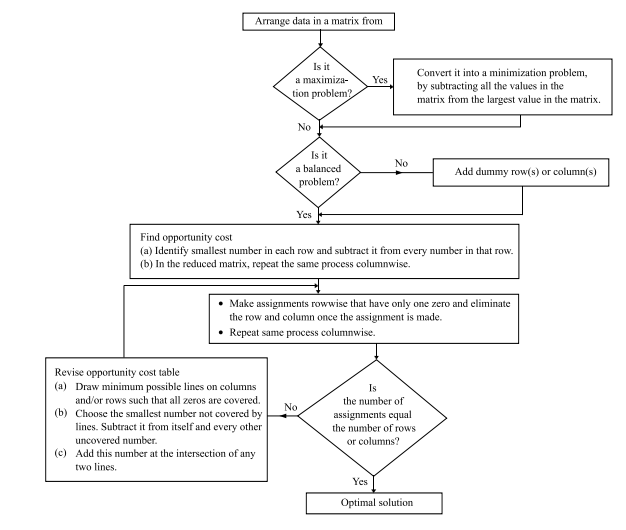
\includegraphics[scale=0.7]{gfx/fig54.png}
\end{center}
\textbf{\textit{Numerical Example:}} Time taken by trucks A, B, C, D, and E to complete jobs 1, 2, 3 , 4, and 5 are given in the table below and each truck is to be assigned a job. Determine the job assignment for each truck such that the time taken to complete all the jobs is minimum.
\begin{center}
	\begin{tabular} {| c | c | c | c | c | c |}
		\hline
		Jobs / Truck & A & B & C & D & E\\
		\hline
		1 & 13 & 8 & 16 & 18 & 19\\
		\hline
		2 & 9 & 15 & 24 & 9 & 12\\
		\hline
		3 & 12 & 9 & 4 & 4 & 4\\
		\hline
		4 & 6 & 12 & 10 & 8 & 13\\
		\hline
		5 & 15 & 17 & 18 & 12 & 20\\
		\hline
	\end{tabular}
\end{center}
\textit{Solution:}\\\\
Rows 1, 2, 3, 4, and 5 have minimum value of 8, 9, 4, 6 , and 12 respectively. Using these values we find out the row reduction matrix.
\begin{center}
	\[\setlength{\arraycolsep}{0pt}
	\begin{NiceArray}{>{\rule[-2.8mm]{0pt}{8mm}}ccccccc}%
		[
		columns-width=8mm ,
		corners = {NW,NE} ,
		hvlines
		]
		& A  & B  & C & D & E \\
		1 & 5 & 0 & 8 & 10 & 11 & \NotEmpty \\
		2 & 0 & 6 & 15 & 0 & 3 & \NotEmpty    \\
		3 & 8 & 5 & 0 & 0 & 0 &               \\
		4 & 0 & 6 & 4 & 2 & 7 & \NotEmpty    \\
		5 & 3 & 5 & 6 & 0 & 8 & \NotEmpty    \\
		&  & & &  \\
		
	\end{NiceArray}\]
\end{center}
Similarly, all the columns have minimum value of 0. Using these values we find out the column reduction matrix.
\begin{center}
	\[\setlength{\arraycolsep}{0pt}
	\begin{NiceArray}{>{\rule[-2.8mm]{0pt}{8mm}}ccccccc}%
		[
		columns-width=8mm ,
		corners = {NW,NE} ,
		hvlines
		]
		& A  & B  & C & D & E \\
		1 & 5 & 0 & 8 & 10 & 11 & \NotEmpty \\
		2 & 0 & 6 & 15 & 0 & 3 & \NotEmpty    \\
		3 & 8 & 5 & 0 & 0 & 0 &               \\
		4 & 0 & 6 & 4 & 2 & 7 & \NotEmpty    \\
		5 & 3 & 5 & 6 & 0 & 8 & \NotEmpty    \\
		&  & & &  \\
		
	\end{NiceArray}\]
\end{center}
Then, rows 1, 4, and 5 have only one 0, so we assign these cells with square bracket and cross out any other value of 0 in the respective columns which have been assigned. Similarly column wise, column C has got only one 0, so we assign that cell and cross out the remaining 0 values in the row corresponding to this assigned cell.
\begin{center}
	\[\setlength{\arraycolsep}{0pt}
	\begin{NiceArray}{>{\rule[-2.8mm]{0pt}{8mm}}ccccccc}%
		[
		columns-width=8mm ,
		corners = {NW,NE} ,
		hvlines
		]
		& A  & B  & C & D & E \\
		1 & 5 & [0] & 8 & 10 & 11 & \NotEmpty \\
		2 & 0 \times & 6 & 15 & 0 \times & 3 & \NotEmpty    \\
		3 & 8 & 5 & [0] & 0 \times & 0 \times &               \\
		4 & [0] & 6 & 4 & 2 & 7 & \NotEmpty    \\
		5 & 3 & 5 & 6 & [0] & 8 & \NotEmpty    \\
		&  & & &  \\
		
	\end{NiceArray}\]
\end{center}
Since there are cost matrix is of size 5 $\times$ 5, we require 5 assignments for the solution to be optimal. However, we have only got 4 assignments, so the solution is not optimal. Now, we should draw minimum number of horizontal and vertical lines such that it covers all zeros to revise the cost matrix for optimal solution.\\
Out of all five rows row 2 is not assigned, so we tick mark this row. In the marked row we have two cells having zero which belongs to column A and D, so we mark these columns. In the marked column A and D we have a cell which consists an assigned 0 for each column, so we mark the rows corresponding to these cells ( row 4 and 5). Now we draw horizontal lines on the rows which has not been marked, and draw vertical lines on the columns which has not been marked.
\begin{center}
	\[\setlength{\arraycolsep}{0pt}
	\begin{NiceArray}{>{\rule[-2.8mm]{0pt}{8mm}}ccccccc}%
		[
		columns-width=8mm ,
		corners = {NW,NE} ,
		hvlines
		]
		& A  & B  & C & D & E \\
		1 & 5 & [0] & 8 & 10 & 11 & \NotEmpty \\
		2 & 0 \times & 6 & 15 & 0 \times & 3 & \checkmark    \\
		3 & 8 & 5 & [0] & 0 \times & 0 \times &               \\
		4 & [0] & 6 & 4 & 2 & 7 & \checkmark    \\
		5 & 3 & 5 & 6 & [0] & 8 & \checkmark  \\
		& \checkmark & & & \checkmark \\
		\CodeAfter \tikz \draw (2.5-|2) -- (2.5-|7)
								(4.5-|2) -- (4.5-|7)
								(2-|2.5) -- (7-|2.5)
								(2-|5.5) -- (7-|5.5);
	\end{NiceArray}\]
\end{center}
For the revised cost matrix we require the value of $ k $, which is the minimum value among the cells which remain uncovered by the lines. In this case, the value of $k$ is 3. Then, we add the value of $k$ to the cell values which lies in the intersection of the drawn lines and subtract the value of $k$ from the cell values which remained uncovered by the lines. Now, the cost matrix has been revised.
\begin{center}
	\[\setlength{\arraycolsep}{0pt}
	\begin{NiceArray}{>{\rule[-2.8mm]{0pt}{8mm}}ccccccc}%
		[
		columns-width=8mm ,
		corners = {NW,NE} ,
		hvlines
		]
		& A  & B  & C & D & E \\
		1 & 8 & 0 & 8 & 13 & 11 & \NotEmpty \\
		2 & 0  & 3 & 12 & 0 & 0 & \NotEmpty    \\
		3 & 11 & 5 & 0 & 3  & 0  &               \\
		4 & 0 & 3 & 1 & 2 & 4 & \NotEmpty    \\
		5 & 3 & 2 & 3 & 0 & 5 & \NotEmpty    \\
		&  & & &  \\
		
	\end{NiceArray}\]
\end{center}
Again rows 1, 4, and 5 have only one cell having the value of 0 (1-B, 4-A,k and 5-D), so we assign these cells with square brackets and cross out the cells having the value of 0 in their respective columns. Similarly column wise column C has only one cell having the value of 0 (3-C), so we assign this cell with square bracket and cross out the cell having the value of 0 in its respective row. 
\begin{center}
	\[\setlength{\arraycolsep}{0pt}
	\begin{NiceArray}{>{\rule[-2.8mm]{0pt}{8mm}}ccccccc}%
		[
		columns-width=8mm ,
		corners = {NW,NE} ,
		hvlines
		]
		& A  & B  & C & D & E \\
		1 & 8 & [0] & 8 & 13 & 11 & \NotEmpty \\
		2 & 0 \times & 3 & 12 & 0 \times & [0] & \NotEmpty    \\
		3 & 11 & 5 &[0] & 3 & 0 \times &               \\
		4 & [0] & 3 & 1 & 2 & 4 & \NotEmpty    \\
		5 & 3 & 2 & 3 & [0] & 5 & \NotEmpty    \\
		&  & & &  \\
		
	\end{NiceArray}\]
\end{center}
$\because$ the size of the matrix = the number of assignments = 5, the solution obtained is the optimal solution.\\
The optimum assignment is given below:
\begin{center}
	\begin{tabular}{| c | c |}
		\hline
		Job & Truck \\
		\hline
		1 & B \\
		\hline
		2 & E \\
		\hline
		3 & C \\
		\hline
		4 & A \\
		\hline
		5 & D \\
		\hline
	\end{tabular}
\end{center}
Also, minimum time = 8 + 12 + 4 + 6 + 12 = 42.
%
\section{Travelling Salesman Problem}
The travelling salesman problem asks the following question: "Given a list of cities and the distances between each pair of cities, what is the shortest possible route that visits each city exactly once and returns to the origin city?".\\\\
Just consider how a postman delivers the post to the addressee. He arranges all the letters in an order and starts from the post office and goes from addressee to addressee and finally back to his post office. If he does not arrange the posts in an order he may have to travel a long distance to clear all the posts. Similarly, a traveling sales man has to plan his visits. Let us say, he starts from his head office and go round the branch offices and come back to his head office. While traveling he will not visit the branch already visited and he will not come back until he visits all the branches.
\\\\
There are different types of traveling salesman's problems. One is \textbf{\textit{cyclic}} problem. In this problem, he starts from his head quarters and after visiting all the branches, he will be back to his head quarters. The second one is \textbf{\textit{Acyclic}} problem. In this case, the traveling salesman leaves his head quarters and after visiting the intermediate branches, finally reaches the last branch and stays there. The first type of the problem is solved by Hungarian method or Assignment technique. The second one is solved by Dynamic programming method.\\\\
\textit{Note: The traveling salesman problem, where we sequence the cities or branches he has to visit is a SEQUENCING PROBLEM. But the solution is solved using the Assignment technique. Hence basically, the traveling salesman problem is a SEQUENCING PROBLEM; the objective is to minimize the total distance traveled.}\\\\
\textbf{\textit{Numerical Example:\\
A salesman stationed at city A has to decide his tour plan to visit cities B, C, D, E and back to city A I the order of his choice so that total distance traveled is minimum. No sub touring is permitted. He cannot travel from city A to city A itself. The distance between cities in Kilometers is given below:}}
\begin{center}
	\begin{tabular}{c | c | c | c | c | c}
		Cities & A & B & C & D & E \\
		\hline
		A & $\infty$ & 16 & 18 & 13 & 20 \\
		\hline
		B & 21 & $\infty$ & 16 & 27 & 14 \\
		\hline
		C & 12 & 14 & $\infty$ & 15 & 21 \\
		\hline
		D & 11 & 18 & 19 & $\infty$ & 21 \\
		\hline
		E & 16 & 14 & 17 & 12 & $\infty$
	\end{tabular}
\end{center}
Solution:\\
Performing row reduction we get the row opportunity cost matrix (ROCM).
\begin{center}
	\[\setlength{\arraycolsep}{0pt}
	\begin{NiceArray}{>{\rule[-2.8mm]{0pt}{8mm}}ccccccc}%
		[
		columns-width=8mm ,
		corners = {NW,NE} ,
		hvlines
		]
		& A  & B  & C & D & E \\
		A & \infty & 3 & 5 & 0 & 7 & \NotEmpty \\
		B & 7  & \infty & 2 & 13 & 0 & \NotEmpty    \\
		C & 0 & 2 & \infty & 3  & 9  &               \\
		D & 0 & 7 & 8 & \infty & 10 & \NotEmpty    \\
		E & 4 & 2 & 5 & 0 & \infty & \NotEmpty    \\
		&  & & &  \\
		
	\end{NiceArray}\]
\end{center}
Performing column reduction on the ROCM we get the total opportunity cost matrix (TOCM).
\begin{center}
	\[\setlength{\arraycolsep}{0pt}
	\begin{NiceArray}{>{\rule[-2.8mm]{0pt}{8mm}}ccccccc}%
		[
		columns-width=8mm ,
		corners = {NW,NE} ,
		hvlines
		]
		& A  & B  & C & D & E \\
		A & \infty & 1 & 3 & 0 & 7 & \NotEmpty \\
		B & 7  & \infty & 0 & 13 & 0 & \NotEmpty    \\
		C & 0 & 0 & \infty & 3  & 9  &               \\
		D & 0 & 5 & 6 & \infty & 10 & \NotEmpty    \\
		E & 4 & 0 & 3 & 0 & \infty & \NotEmpty    \\
		&  & & &  \\
		
	\end{NiceArray}\]
\end{center}
Now we assign using the same technique used in the Assignment Problem.
\begin{center}
	\[\setlength{\arraycolsep}{0pt}
	\begin{NiceArray}{>{\rule[-2.8mm]{0pt}{8mm}}ccccccc}%
		[
		columns-width=8mm ,
		corners = {NW,NE} ,
		hvlines
		]
		& A  & B  & C & D & E \\
		A & \infty & 1 & 3 & [0] & 7 & \NotEmpty \\
		B & 7  & \infty & [0] & 13 & 0 \times & \NotEmpty    \\
		C & 0 \times & 0 \times & \infty & 3  & 9  &               \\
		D & [0] & 5 & 6 & \infty & 10 & \NotEmpty    \\
		E & 4 & [0] & 3 & 0 \times & \infty & \NotEmpty    \\
		&  & & &  \\
		
	\end{NiceArray}\]
\end{center}
Since we there are only 4 assignments but the matrix is of size 5 $\times$ 5, we need to modify the opportunity cost matrix for optimum solution. Now, we will draw the minimum number of vertical and horizontal lines to cover all the 0's.
\begin{center}
	\[\setlength{\arraycolsep}{0pt}
	\begin{NiceArray}{>{\rule[-2.8mm]{0pt}{8mm}}ccccccc}%
		[
		columns-width=8mm ,
		corners = {NW,NE} ,
		hvlines
		]
		& A  & B  & C & D & E \\
		A & \infty & 1 & 3 & [0] & 7 & \checkmark \\
		B & 7  & \infty & [0] & 13 & 0 \times & \NotEmpty    \\
		C & 0 \times & 0 \times & \infty & 3  & 9  &  \checkmark             \\
		D & [0] & 5 & 6 & \infty & 10 & \checkmark    \\
		E & 4 & [0] & 3 & 0 \times & \infty & \checkmark    \\
		& \checkmark & \checkmark& & \checkmark \\
		\CodeAfter \tikz \draw (3.5-|2) -- (3.5-|7)
								(2-|2.5) -- (7-|2.5)
								(2-|3.5) -- (7-|3.5)
								(2-|5.5) -- (7-|5.5);
	\end{NiceArray}\]
\end{center}
For new opportunity cost matrix, k = min(3, 6, 7, 9, $\infty$) = 3. The new opportunity cost matrix is:
\begin{center}
	\[\setlength{\arraycolsep}{0pt}
	\begin{NiceArray}{>{\rule[-2.8mm]{0pt}{8mm}}ccccccc}%
		[
		columns-width=8mm ,
		corners = {NW,NE} ,
		hvlines
		]
		& A  & B  & C & D & E \\
		A & \infty & 1 & 0 & 0 & 4 & \NotEmpty \\
		B & 10  & \infty & 0 & 16 & 0 & \NotEmpty    \\
		C & 0  & 0  & \infty & 3  & 6  &               \\
		D & 0 & 5 & 3 & \infty & 7 & \NotEmpty    \\
		E & 4 & 0 & 0 & 0 \times & \infty & \NotEmpty    \\
		&  & & &  \\
		
	\end{NiceArray}\]
\end{center}
Again we assign the cells for the solution.
\begin{center}
	\[\setlength{\arraycolsep}{0pt}
	\begin{NiceArray}{>{\rule[-2.8mm]{0pt}{8mm}}ccccccc}%
		[
		columns-width=8mm ,
		corners = {NW,NE} ,
		hvlines
		]
		& A  & B  & C & D & E \\
		A & \infty & 1 & 0 & 0 & 4 & \NotEmpty \\
		B & 10  & \infty & 0 \times & 16 & [0] \times & \NotEmpty    \\
		C & 0 \times & [0]  & \infty & 3  & 6  &               \\
		D & [0] & 5 & 3 & \infty & 7 & \NotEmpty    \\
		E & 4 & 0 \times & 0 & 0  & \infty & \NotEmpty    \\
		&  & & &  \\
		
	\end{NiceArray}\]
\end{center}
Here we have a tie situation, that is, more than one solution can be obtained. At first we assign the cell A-D, we get:
\begin{center}
	\[\setlength{\arraycolsep}{0pt}
	\begin{NiceArray}{>{\rule[-2.8mm]{0pt}{8mm}}ccccccc}%
		[
		columns-width=8mm ,
		corners = {NW,NE} ,
		hvlines
		]
		& A  & B  & C & D & E \\
		A & \infty & 1 & 0 \times & [0] & 4 & \NotEmpty \\
		B & 10  & \infty & 0 \times & 16 & [0] \times & \NotEmpty    \\
		C & 0 \times & [0]  & \infty & 3  & 6  &               \\
		D & [0] & 5 & 3 & \infty & 7 & \NotEmpty    \\
		E & 4 & 0 \times & [0] & 0 \times & \infty & \NotEmpty    \\
		&  & & &  \\
		
	\end{NiceArray}\]
\end{center}
We have got 5 assignments, however, the solution is not valid for TSP since there are two cycles, that is, (A $\rightarrow$ D, D $\rightarrow$ A) and ( B $\rightarrow$ E, E $\rightarrow$ C, C $\rightarrow$ B ).\\\\
Now, we assign the cell A-C, we get:
\begin{center}
	\[\setlength{\arraycolsep}{0pt}
	\begin{NiceArray}{>{\rule[-2.8mm]{0pt}{8mm}}ccccccc}%
		[
		columns-width=8mm ,
		corners = {NW,NE} ,
		hvlines
		]
		& A  & B  & C & D & E \\
		A & \infty & 1 & [0] & 0 \times & 4 & \NotEmpty \\
		B & 10  & \infty & 0 \times & 16 & [0] \times & \NotEmpty    \\
		C & 0 \times & [0]  & \infty & 3  & 6  &               \\
		D & [0] & 5 & 3 & \infty & 7 & \NotEmpty    \\
		E & 4 & 0 \times & 0 \times  & [0]  & \infty & \NotEmpty    \\
		&  & & &  \\
		
	\end{NiceArray}\]
\end{center}
We have 5 assignments, and the solution is valid for TSP since it makes a one complete cycle travelling all cities starting from city A (A $\rightarrow$ C, C $\rightarrow$ B, B $\rightarrow$ E, E $\rightarrow$ D, D $\rightarrow$ A). \\
The minimum distance = 18 + 14 + 14 + 12 + 11 = 69 Km.\\\\
\textbf{\textit{Numerical Example: \\
Given the travel costs below, show how to sequence the travel between the cities so as to minimize the total setup cost per cycle.}}
\begin{center}
	\begin{tabular}{c | c | c | c | c | c}
		Cities & A & B & C & D & E \\
		\hline
		A & $\infty$ & 2 & 5 & 7 & 1 \\
		\hline
		B & 6 & $\infty$ & 3 & 8 & 2 \\
		\hline
		C & 8 & 7 & $\infty$ & 4 & 7 \\
		\hline
		D & 12 & 4 & 6 & $\infty$ & 5 \\
		\hline
		E & 1 & 3 & 2 & 8 & $\infty$
	\end{tabular}
\end{center}
Solution:\\
ROCM:
\begin{center}
	\[\setlength{\arraycolsep}{0pt}
	\begin{NiceArray}{>{\rule[-2.8mm]{0pt}{8mm}}ccccccc}%
		[
		columns-width=8mm ,
		corners = {NW,NE} ,
		hvlines
		]
		& A  & B  & C & D & E \\
		A & \infty & 1 & 4 & 6 & 0 & \NotEmpty \\
		B & 4  & \infty & 1 & 6 & 0 & \NotEmpty    \\
		C & 4 & 3 & \infty & 0  & 3  &               \\
		D & 8 & 0 & 2 & \infty & 1 & \NotEmpty    \\
		E & 0 & 2 & 1 & 7 & \infty & \NotEmpty    \\
		&  & & &  \\
		
	\end{NiceArray}\]
\end{center}
TOCM:
\begin{center}
	\[\setlength{\arraycolsep}{0pt}
	\begin{NiceArray}{>{\rule[-2.8mm]{0pt}{8mm}}ccccccc}%
		[
		columns-width=8mm ,
		corners = {NW,NE} ,
		hvlines
		]
		& A  & B  & C & D & E \\
		A & \infty & 1 & 3 & 6 & 0 & \NotEmpty \\
		B & 4  & \infty & 0 & 6 & 0 & \NotEmpty    \\
		C & 4 & 3 & \infty & 0  & 3  &               \\
		D & 8 & 0 & 1 & \infty & 1 & \NotEmpty    \\
		E & 0 & 2 & 0 & 7 & \infty & \NotEmpty    \\
		&  & & &  \\
		
	\end{NiceArray}\]
\end{center}
Now, we assign the cells for the solution.
\begin{center}
	\[\setlength{\arraycolsep}{0pt}
	\begin{NiceArray}{>{\rule[-2.8mm]{0pt}{8mm}}ccccccc}%
		[
		columns-width=8mm ,
		corners = {NW,NE} ,
		hvlines
		]
		& A  & B  & C & D & E \\
		A & \infty & 1 & 3 & 6 & [0] & \NotEmpty \\
		B & 4  & \infty & [0] & 6 & 0 \times & \NotEmpty    \\
		C & 4 & 3 & \infty & [0]  & 3  &               \\
		D & 8 & [0] & 1 & \infty & 1 & \NotEmpty    \\
		E & [0] & 2 & 0 \times & 7 & \infty & \NotEmpty    \\
		&  & & &  \\
		
	\end{NiceArray}\]
\end{center}
We have got 5 assignments, however, the solution is not valid for TSP since there are two cycles, that is, (A $\rightarrow$ E, E $\rightarrow$ A) and ( B $\rightarrow$ C, C $\rightarrow$ D, D $\rightarrow$ B ).\\\\
The next best solution is obtained by assigning minimum non-zero cell in the matrix ( In this case 1). At first, we have to assign all 1's and then the 0's. Also we have a tie between the cells D-C and D-E. At first, we assign the cell D-C.
\begin{center}
	\[\setlength{\arraycolsep}{0pt}
	\begin{NiceArray}{>{\rule[-2.8mm]{0pt}{8mm}}ccccccc}%
		[
		columns-width=8mm ,
		corners = {NW,NE} ,
		hvlines
		]
		& A  & B  & C & D & E \\
		A & \infty & [1] & 3 & 6 & 0 \times & \NotEmpty \\
		B & 4  & \infty & 0 \times & 6 & [0] & \NotEmpty    \\
		C & 4 & 3 & \infty & [0]  & 3  &               \\
		D & 8 & 0 \times & [1] & \infty & 1 \times & \NotEmpty    \\
		E & [0] & 2 & 0 \times & 7 & \infty & \NotEmpty    \\
		&  & & &  \\
		
	\end{NiceArray}\]
\end{center}
We have got 5 assignments, however, the solution is not valid for TSP since there are two cycles, that is, (C $\rightarrow$ D, D $\rightarrow$ C) and (A $\rightarrow$ B, B $\rightarrow$ E, E $\rightarrow$ A ).\\\\
Now, we assign the cell D-E.
\begin{center}
	\[\setlength{\arraycolsep}{0pt}
	\begin{NiceArray}{>{\rule[-2.8mm]{0pt}{8mm}}ccccccc}%
		[
		columns-width=8mm ,
		corners = {NW,NE} ,
		hvlines
		]
		& A  & B  & C & D & E \\
		A & \infty & [1] & 3 & 6 & 0 \times & \NotEmpty \\
		B & 4  & \infty & [0] & 6 & 0 \times & \NotEmpty    \\
		C & 4 & 3 & \infty & [0]  & 3  &               \\
		D & 8 & 0 \times & 1 \times & \infty & [1] & \NotEmpty    \\
		E & [0] & 2 & 0 \times & 7 & \infty & \NotEmpty    \\
		&  & & &  \\
		
	\end{NiceArray}\]
\end{center}
We have 5 assignments, and the solution is valid for TSP since it makes a one complete cycle travelling all cities starting from city A (A $\rightarrow$ B, B $\rightarrow$ C, C $\rightarrow$ D, D $\rightarrow$ E, E $\rightarrow$ A). \\
minimum distance = 2 + 3 + 4 + 5 + 1 = 15
%
\section{Review Problems}
\begin{enumerate}
	\item Describe the three main actors involved in freight transportation and distribution.
	\item List out the factors that influences the decision of shippers regarding the choice of carrier and transportation mode.
	\item Describe the two ways in which shipments can be made.
	\item Describe the three distribution structures used in freight transport and distribution.
	\item Write the differences among the North-West Corner Method, Least-Cost Cell Method, and Vogel's Approximation Method.
	\item A dairy firm has three plants located in a state. The daily milk production at each plant is as follows: Plant 1 : 6 million litres, Plant 2 : 1 million litres, and Plant 3 : 10 million litres.\\\\
	Each day, the firm must fulfil the needs of its four distribution centres. The minimum requirement of each centre is as follows: Distribution centre 1 : 7 million litres, Distribution centre 2 : 5 million litres, Distribution centre 3 : 3 million litres, and Distribution centre 4 : 2 million litres.\\\\
	Cost (in hundreds of rupees) of shipping one million litre from each plant to each distribution centre is given
	in the following table:
		\begin{center}
			\begin{tabular}{c | c | c | c | c}
				Plant / Distribution Center & $D_1$ & $D_2$ & $D_3$ & $D_4$\\
				\hline
				$P_1$ & 2 & 3 & 11 & 7\\
				\hline
				$P_2$ & 1 & 0 & 6 & 1 \\
				\hline
				$P_3$ & 5 & 8 & 15 & 9
			\end{tabular}
		\end{center}
	Find the initial basic feasible solution for given problem by using following methods:
		\begin{enumerate}
			\item North-West Corner Method
			\item Least-Cost Cell Method
			\item Vogel's Approximation Method
		\end{enumerate}
	\item A  logistics department of a freight company has five trucks with five jobs to be performed. The time (in hours) that each truck takes to perform each job is given in the effectiveness matrix.
		\begin{center}
			\begin{tabular}{c | c | c | c | c | c}
				Job / Truck & 1 & 2 & 3 & 4 & 5\\
				\hline
				A & 10 & 5 & 13 & 15 & 16 \\
				\hline
				B & 3 & 9 & 18 & 13 & 6 \\
				\hline
				C & 10 & 7 & 2 & 2 & 2 \\
				\hline
				D & 7 & 11 & 9 & 7 & 12 \\
				\hline
				E & 7 & 9 & 10 & 4 & 12
			\end{tabular}
		\end{center}
	How should the jobs be allocated, one per truck, so as to minimize the total truck-hours?
	\item An Online Delivery organization is planning to deliver packages to 5 cities. Starting from the head office at city A then going round B, C, D and E and then come back to A. Their objective is to minimize the total distance covered. Help them in sequencing the cities. A, B, C, D and E as the shown in the figure. The numbers on the arrows show the distances in Km.
		\begin{center}
			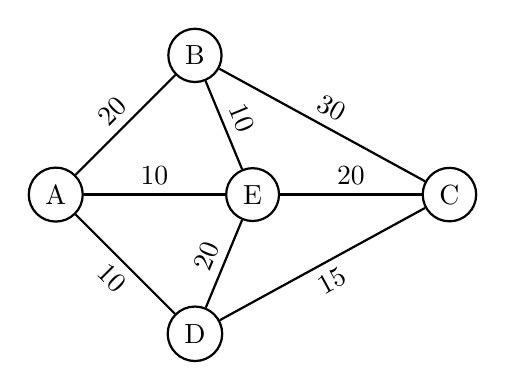
\begin{tikzpicture}[node distance={25mm}, thick, main/.style = {draw, circle}]
				\node[main] (1) {A};
				\node[main] (2) [right of = 1] {E};
				\node[main] (3) [above right of = 1] {B};
				\node[main] (4) [below right of = 1] {D};
				\node[main] (5) [right of = 2] {C};
				\draw(1) -- node[midway, above ] {10} (2);
				\draw(2) -- node[midway, above ] {20} (5);
				\draw(1) -- node[midway, above, sloped ] {20} (3);
				\draw(1) -- node[midway, below, sloped ] {10} (4); 
				\draw(2) -- node[midway, above, sloped ] {10} (3);
				\draw(2) -- node[midway, above, sloped ] {20} (4);
				\draw(3) -- node[midway, above, sloped ] {30} (5);
				\draw(4) -- node[midway, below, sloped ] {15} (5);
			\end{tikzpicture}
		\end{center}
\end{enumerate}
%
\subsection{Answers}
\begin{description}
	\item [6]. \begin{description}
		\item [a] $x_{11} = 6$, $x_{21} = 1$, $x_{32} = 5$, $x_{33} = 3$, $x_{34} = 2$, and Total Cost = Rs. 11600
		\item [b] $x_{11} = 6$, $x_{22} = 1$, $x_{31} = 1$, $x_{32} = 4$, $x_{33} = 3$, $x_{34} = 2$, and Total Cost = Rs. 11200
		\item [c] $x_{11} = 1$, $x_{12} = 5$, $x_{24} = 1$, $x_{31} = 6$, $x_{33} = 3$, $x_{34} = 1$, and Total Cost = Rs. 10200
	\end{description}
	\item [7]. \begin{center}
		\begin{tabular}{| c | c | c |}
			\hline
			Job & Truck & Time\\
			\hline
			A & 2 & 5\\
			\hline
			B & 1 & 3\\ 
			\hline
			C & 5 & 2\\ 
			\hline
			D & 3 & 9\\ 
			\hline
			E & 4 & 4\\ 
			\hline
			& & Total = 23
		\end{tabular}
	\end{center}
	\item [8]. The shortest route is (A $\rightarrow$ E, E $\rightarrow$ D, D $\rightarrow$ C, C $\rightarrow$ B, B $\rightarrow$ A) and the distance travelled = 95 Km.
\end{description}